\documentclass[thesis=M,english]{FITthesis}[2012/10/20]

% graphics files inclusion
\usepackage{graphicx}
% subfigures
\usepackage{subfig}
% advanced maths
\usepackage{amsmath}
% additional math symbols
\usepackage{amssymb}
% directory tree visualisation
\usepackage{dirtree}

\department{Department of Applied Mathematics}
\title{Neural Networks Based Domain Adaptation in Spectroscopic Sky Surveys}
\authorGN{Ondřej}
\authorFN{Podsztavek}
% author's name without academic degrees
\author{Ondřej Podsztavek}
\authorWithDegrees{Bc. Ondřej Podsztavek}
\supervisor{Petr Škoda}
% TODO acknowledgements
\acknowledgements{}
% TODO english abstract
\abstractEN{}
% TODO czech abstract
\abstractCS{}
\placeForDeclarationOfAuthenticity{Prague}
% TODO english keywords
\keywordsEN{domain adaptation, neural networks, astronomy, spectroscopy}
% TODO czech keywords
\keywordsCS{}
% select according to the desired license (integer 1-6)
\declarationOfAuthenticityOption{2}
% TODO optional thesis URL
%\website{}

\begin{document}

\chapter{Introduction}

How to use neural network based domain adaptation to extract knowledge from the source domain of astronomical spectral data
and apply it to the target astronomical spectral data?

In this work, we would like to prove that astronomical spectroscopy can benefit from domain adapatation (DA).
Previous research has shown that DA can overcome the problem of analysis data from different distribution in one experiment.
In the first chapter~\ref{da_chapter}, we provide a summary of theory of DA, neural networks in DA and DA in astronomy.
Then, in chapter~\ref{data_chapter}, we describe current spectroscopic sky surveys
which might be source of suitable astronomical spectral data.
In experiments~\ref{exp_chapter}, we try to show the benefits of neural DA in astronomy.
Consider that our work is limited to astronomical spectroscopy and neural models.
Having said that, we will apply these methods\dots{}

\section{Problem Definition and Motivation}

The goal of this thesis is the analysis of the impact of domain adaptation in astronomical archives with a focus on neural networks
that would allow using labelled data from one ground-based telescope or space mission archive to discover knowledge in another archive.
Current astronomy has been the primary customer of scalable Big data handling and analysis requirements due to its petabyte-scale archives,
where an advanced machine learning is an indispensable part of workflows leading to new discoveries.

\chapter{Domain Adaptation (DA)}
\label{da_chapter}

Survey the current state of domain adaptation using neural network models in machine learning and with a focus on astronomical applications.

\section{DA in Context of Machine and Transfer Learning}

Now, we introduce the crucial concept of our work: domain adaptation.
Domain adaptation is a subfield of transfer learning,
which is part of machine learning.
Transfer learning is defined in most papers regarding the survey by Pan and Yang~\cite{pan2010}.
A more recent survey by Weiss, Khoshgoftaar and Wang~\cite{weiss2016} has the benefit
that it contains newer methods than the survey by Pan and Yang~\cite{pan2010},
but its definition of transfer learning and domain adaptation is the same.

Machine learning has a common assumption that training and test data are independent and identically distributed
that means samples are drawn from the same feature space and the same distribution.~\cite{daume2006}
When this assumption does not hold transfer learning and domain adaptation come into play.
Moreover, there is a biological inspiration
because humans seem to have natural ways to transfer knowledge from previous experience to new challenges.~\cite{torrey2010}

Pan and Yang define transfer learning as the ability of a system to recognise and apply knowledge and skill learned in previous tasks to novel tasks
and they introduce the notion of a domain and a task.
A domain consists of two components: a feature space and a marginal probability distribution.
Given a specific domain, a task consists of two components: a label space and an objective predictive function
which is not observed but learned from training data.
When we are given a transfer learning problem,
we have to identify a source domain and a source learning task,
a target domain and a target learning task.
Then, transfer learning aims to help improve the learning of the target predictive function in the target domain using knowledge in the source domain and the source task,
where the domains are different or the tasks are different.~\cite{pan2010}

Lastly, Torrey and Shavlik warn that both the source and target domains and tasks need to be sufficiently related
else negative transfer may occur.
Negative transfer is the situation in which the usage of source data degrades the performance.
On the other side, when the performance is improved,
we talk about a positive transfer.~\cite{torrey2010}

\section{Theory and Formalization of DA}

Domain adaptation is the scenario when the source and target domains have different marginal probability distributions
(for example two different telescopes observed the spectra)
while the tasks are the same
(we would like to classify them into the same classes).

\section{Neural Networks in DA}

\section{Previous Applications of DA in Astronomy}

As we have shown, domain adaptation is of great interest to astronomers
because of different instruments, measurements and observation distribution.
Therefore, we survey the current state of domain adaptation in astronomical applications in this section.

If we have a common set of observed stars in both archives,
then we can map them and learn a transfer function.
Ho et al.~\cite{ho2017} did exactly that
% TODO add APOGEE to acronyms
because they found a common set of 9952 spectra in both APOGEE and LAMOST archive.
Using that set, they trained the Cannon method~\cite{ness2015},
and they used the model to transfer some physical parameters from APOGEE to LAMOST.

In the case, when there is no common set Gupta et al. experimented with subspace alignment~\cite{fernando2014} and kernel mean matching~\cite{gretton2009} followed by active learning.~\cite{gupta2016}
In the case of subspace alignment, the negative transfer occurred while the kernel mean matching seems very promising in the task of supernova classification.
Then, Vilalta et al.~\cite{vilalta2018} extended the work of Gupta et al.~\cite{gupta2016}.
Vilalta et al. used a maximum a posteriori (MAP) approach to learn a prior on the model parameters from a spectroscopic source domain
and then use this prior distribution to learn a model in a photometric target domain.
Concretely, Vilalta et al. put a prior on the number of layers of a neural network
and then used active learning.
Richards et al.~\cite{richards2011} faced a similar situation, as Gupta et al.
Richards et al. introduce the problem as sample selection bias~\cite{shimodaira2000} or covariate shift~\cite{heckman1979}
when different distributions generate the source and target data.
That is precisely the problem we have defined as domain adaptation.
Richards et al. experimented with random forest in combination with three domain adaptation methods:
importance weighting~\cite{shimodaira2000}, co-training~\cite{blum1998} and active learning~\cite{settles2009}.
The result is not surprising from our point of view.
Active learning works best while importance weighting and co-training achieve negative transfer.

The term transfer learning has been recently used in the context of deep learning.
However, transfer learning in the context of deep learning means something more concrete than what we defined as transfer learning previously.
Transfer learning in the context of deep learning is the specific situation
when a pretrained deep neural network model is taken,
and its last layers are retrained with the target domain data.
Ackermann et al.~\cite{ackermann2018} employed with the transfer learning approach in the context of deep learning to detect galaxy merges.
Ackermann et al. took the Xception convolutional neural network~\cite{chollet2017}
and retrain its last layers with images of galaxy merger labelled in a citizen science Galaxy Zoo project.
This transfer learning approach allowed Ackermann et al. to lower the best error rate so far by 15\%.

\chapter{Spectroscopic Sky Surveys}
\label{data_chapter}

% TODO chapter summary

Select suitable dataset of astronomical spectra for experiments.

To understand this work we need first to introduce the spectral
data because we are interested in classifying them.

\section{Astronomical Spectroscopy}

Almost all we know about the universe outside our solar solar is based on the analysis of electromagnetic radiation.
We have derived information by observing flux, time variations, etc.~\cite{appenzeller2012}

Light is an electromagnetic wave that can be decomposed (by a prism or a diffraction grating) as a function of its wavelength.
The decomposition is called spectrum.
Electromagnetic wave propagetes in the speed of light \(c\).
The electromagnetic wave transfers energy
(the higher the frequency the more energy it carries).~\cite{cochard2018}

Secondly, light is a beam of photons: particles of light.
Photons has no mass but transport energy and have momentum.
Every photon has an associated frequency \(\nu\) of the corresponding electromagnetic wave giving it a energy \(E = h \nu\).

Matter is made of atoms.
An atom has a specific number of electrons which are place in particular orbits of the atom.
Electrons in an orbit have a specic energy level.
We know from quantum mechanics that an electron can change energy level by an exchange of energy in form of a photon.
The energy transfer is not continuous.
The energy has to precisily correspond to the difference in the energy levels.
Therefore the change produces a light with an energy \(E\) in the wavelegth \(\lambda\):

\begin{equation}
	\lambda = c \frac{h}{E}.
\end{equation}

Therefore, the specific set of energy levels of a atom detemines photons either abosrbed or emitted by it.
This is a direct consequence for spectroscopy.~\cite{cochard2018}

Black body radiation.
Light is produced by either heating up matter or by exciting atoms.
Heating transforms into an emission of light at all wavelenghts with an energy distribution (a function of wavelength) which only depends on the temperature.
Planck's law:

% https://en.wikipedia.org/wiki/Planck%27s_law
\begin{equation}
	B_{\lambda}(\lambda, T) = \frac{2 h c^2}{\lambda^5} \frac{1}{e^{\frac{hc}{\lambda k_{\mathrm{B}}T}} - 1}
\end{equation}

where \(k_{\mathrm{B}}\) is the Boltzmann constant.
This phenomenon does not depend on the composition of the body.
The Wien's displacement law gives the wavelenght of maximum intensity \(\lambda_{\max}\):

\begin{equation}
	\lambda_{\max} = \frac{b}{T}
\end{equation}

where \(b\) is the Wien's displacement constant.
Similarly, we can derive the temperature \(T\) with known wavelength of maximum intesity \(\lambda_{\max}\):

\begin{equation}
	T = \frac{b}{\lambda_{\max}}.
\end{equation}

where \(b\) is the Wien's displacement constant.~\cite{cochard2018}

Secondly, light can be emitted by exciting atoms.

Photons carry information about the observed object to a pixel of a \textit{charge-coupled device} (CCD) camera. % TODO add CCD to acronyms
Electomagnetic radiation exhibits both wave and particle nature throughout the entire spectra
(\(\gamma\) rays, X-rays, ultraviolet, visible light, infrared radiation, microwaves, radio waves).
CCD cameras require the particle nature of light (electromagnetic radiation).~\cite{trypsteen2017}

Maybe include Table~1.3 from~\cite{trypsteen2017}.

A photon caries a specific energy that match certain frequency.
Higher frequency means higher energy.
All photons always move in the speed of light.
For each wavelength the corresponding photon energy \(E\) is given by the Planck--Einstein relation:

\begin{equation}
	E = h \nu \label{planck_einstein_equation}
\end{equation}

where \(h\) is the Planck constant and \(\nu\) is frequency of the photon.
The frequency \(\nu\) is related to the wavelength \(\lambda\):

\begin{equation}
	\nu = \frac{c}{\lambda} \label{frequency_wavelength_equation}
\end{equation}

where \(c\) is the speed of light.
Combining equations~\ref{planck_einstein_equation} and \ref{frequency_wavelength_equation} gives:

\begin{equation}
	E = h \frac{c}{\lambda}.
\end{equation}

Therefore, the energy of a photon is proportional to its frequency \(\nu\)
and inversly proportional to the wavelength \(\lambda\).~\cite{trypsteen2017}

The blackbody is a physical model for stellar radiation.
Objects hotter than its environment emit electromagnetic radiation.
Objects also reflect radiation.
But stars rather absorb all incomming radiation.
Therefore, we consider the Sun as a blackbody.
A perfert blackbody absorbs all incomming radiation.
Therefore, all its radiation is determined only by its temperature.~\cite{trypsteen2017}

The undisturbed profile of a continuum level \(I_C(\lambda)\) represents roughly the temperature dependence blackbody radiation characteristics \(B_T(\lambda)\).

With the Wien's displacement law we can estimate the absolute temperature \(T\) of a star.

Bolometric energy flow \(F_{\mathrm{bol}}\):

\begin{equation}
	F_{\mathrm{bol}} = \int_0^{\infty} I(\lambda) \mathrm{d} \lambda
\end{equation}

and Stefan--Bolzmann law:

\begin{equation}
	F_{\mathrm{bol}} = \sigma T^4
\end{equation}

where \(\sigma\) is the Stefan--Bolzmann constant.~\cite{trypsteen2017}

Telescopes are giant eyes that can collect much more light that human's eye.
Spectrographs can disperse the light collected by a telescope into spectra
which reveal objects composition, speed, temperature and more.~\cite{bennett2005}

The visible light is only a tiny part of the complete spectrum of electromagnetic radiation.
The complete spectrum of electromagnetic radiation is usually called the electromagnetic spectrum.
Electromagnetic radiation carries information about stars and planets made of matter across the universe.
The energy carried by light interacts with matter in following ways:

\begin{itemize}
	\item \textit{emission} (an electric current flowing through the bulb heats it to a point at
		which its matter emits visible light);
	\item \textit{absorption} (hand placed near a lit light bulb absorbs some of the light).
\end{itemize}

Spectra come in three basic types, and real astronomical spectra are usually a combination of these types:

\begin{itemize}
	\item the spectrum of a conventional light bulb is a continuous rainbow (called \textit{thermal radiation spectrum});
	\item if a cloud of gas lies between a detector and a bulb,
		the cloud can absorb specific wavelength making what an absorption line spectrum;
	\item the cloud might emit light itself; therefore, this spectrum is called an emission-line spectrum.
\end{itemize}

The fact that each atom, ion or molecule possesses a unique set of energy levels
causes emission and absorption lines at specific wavelengths in spectra.
Spectral lines correspond to the wavelengths of light absorbed by chemicals on the surface of the star.
Therefore, positions of emission and absorption lines can tell us objects composition.
We display spectra as bands of light that is a projection of light that passes through a prism on a wall
(see Fig.~\ref{solar_spectrum}):
called \textit{two dimensional} spectra.~\cite{cochard2018}
A more reasonable way is to display spectra as graphs of intensities of the light as the vertical axis and wavelengths as the horizontal axis:
called a \textit{one-dimensional spectral profile}.~\cite{cochard2018}
This representation of a astronomical spectrum can be seen as a one-dimensional image.
Therefore, convolutional neural networks seem to be a great tool to analyse them.~\cite{bennett2005}

\begin{figure}
	% source https://solarsystem.nasa.gov/resources/390/the-solar-spectrum/
	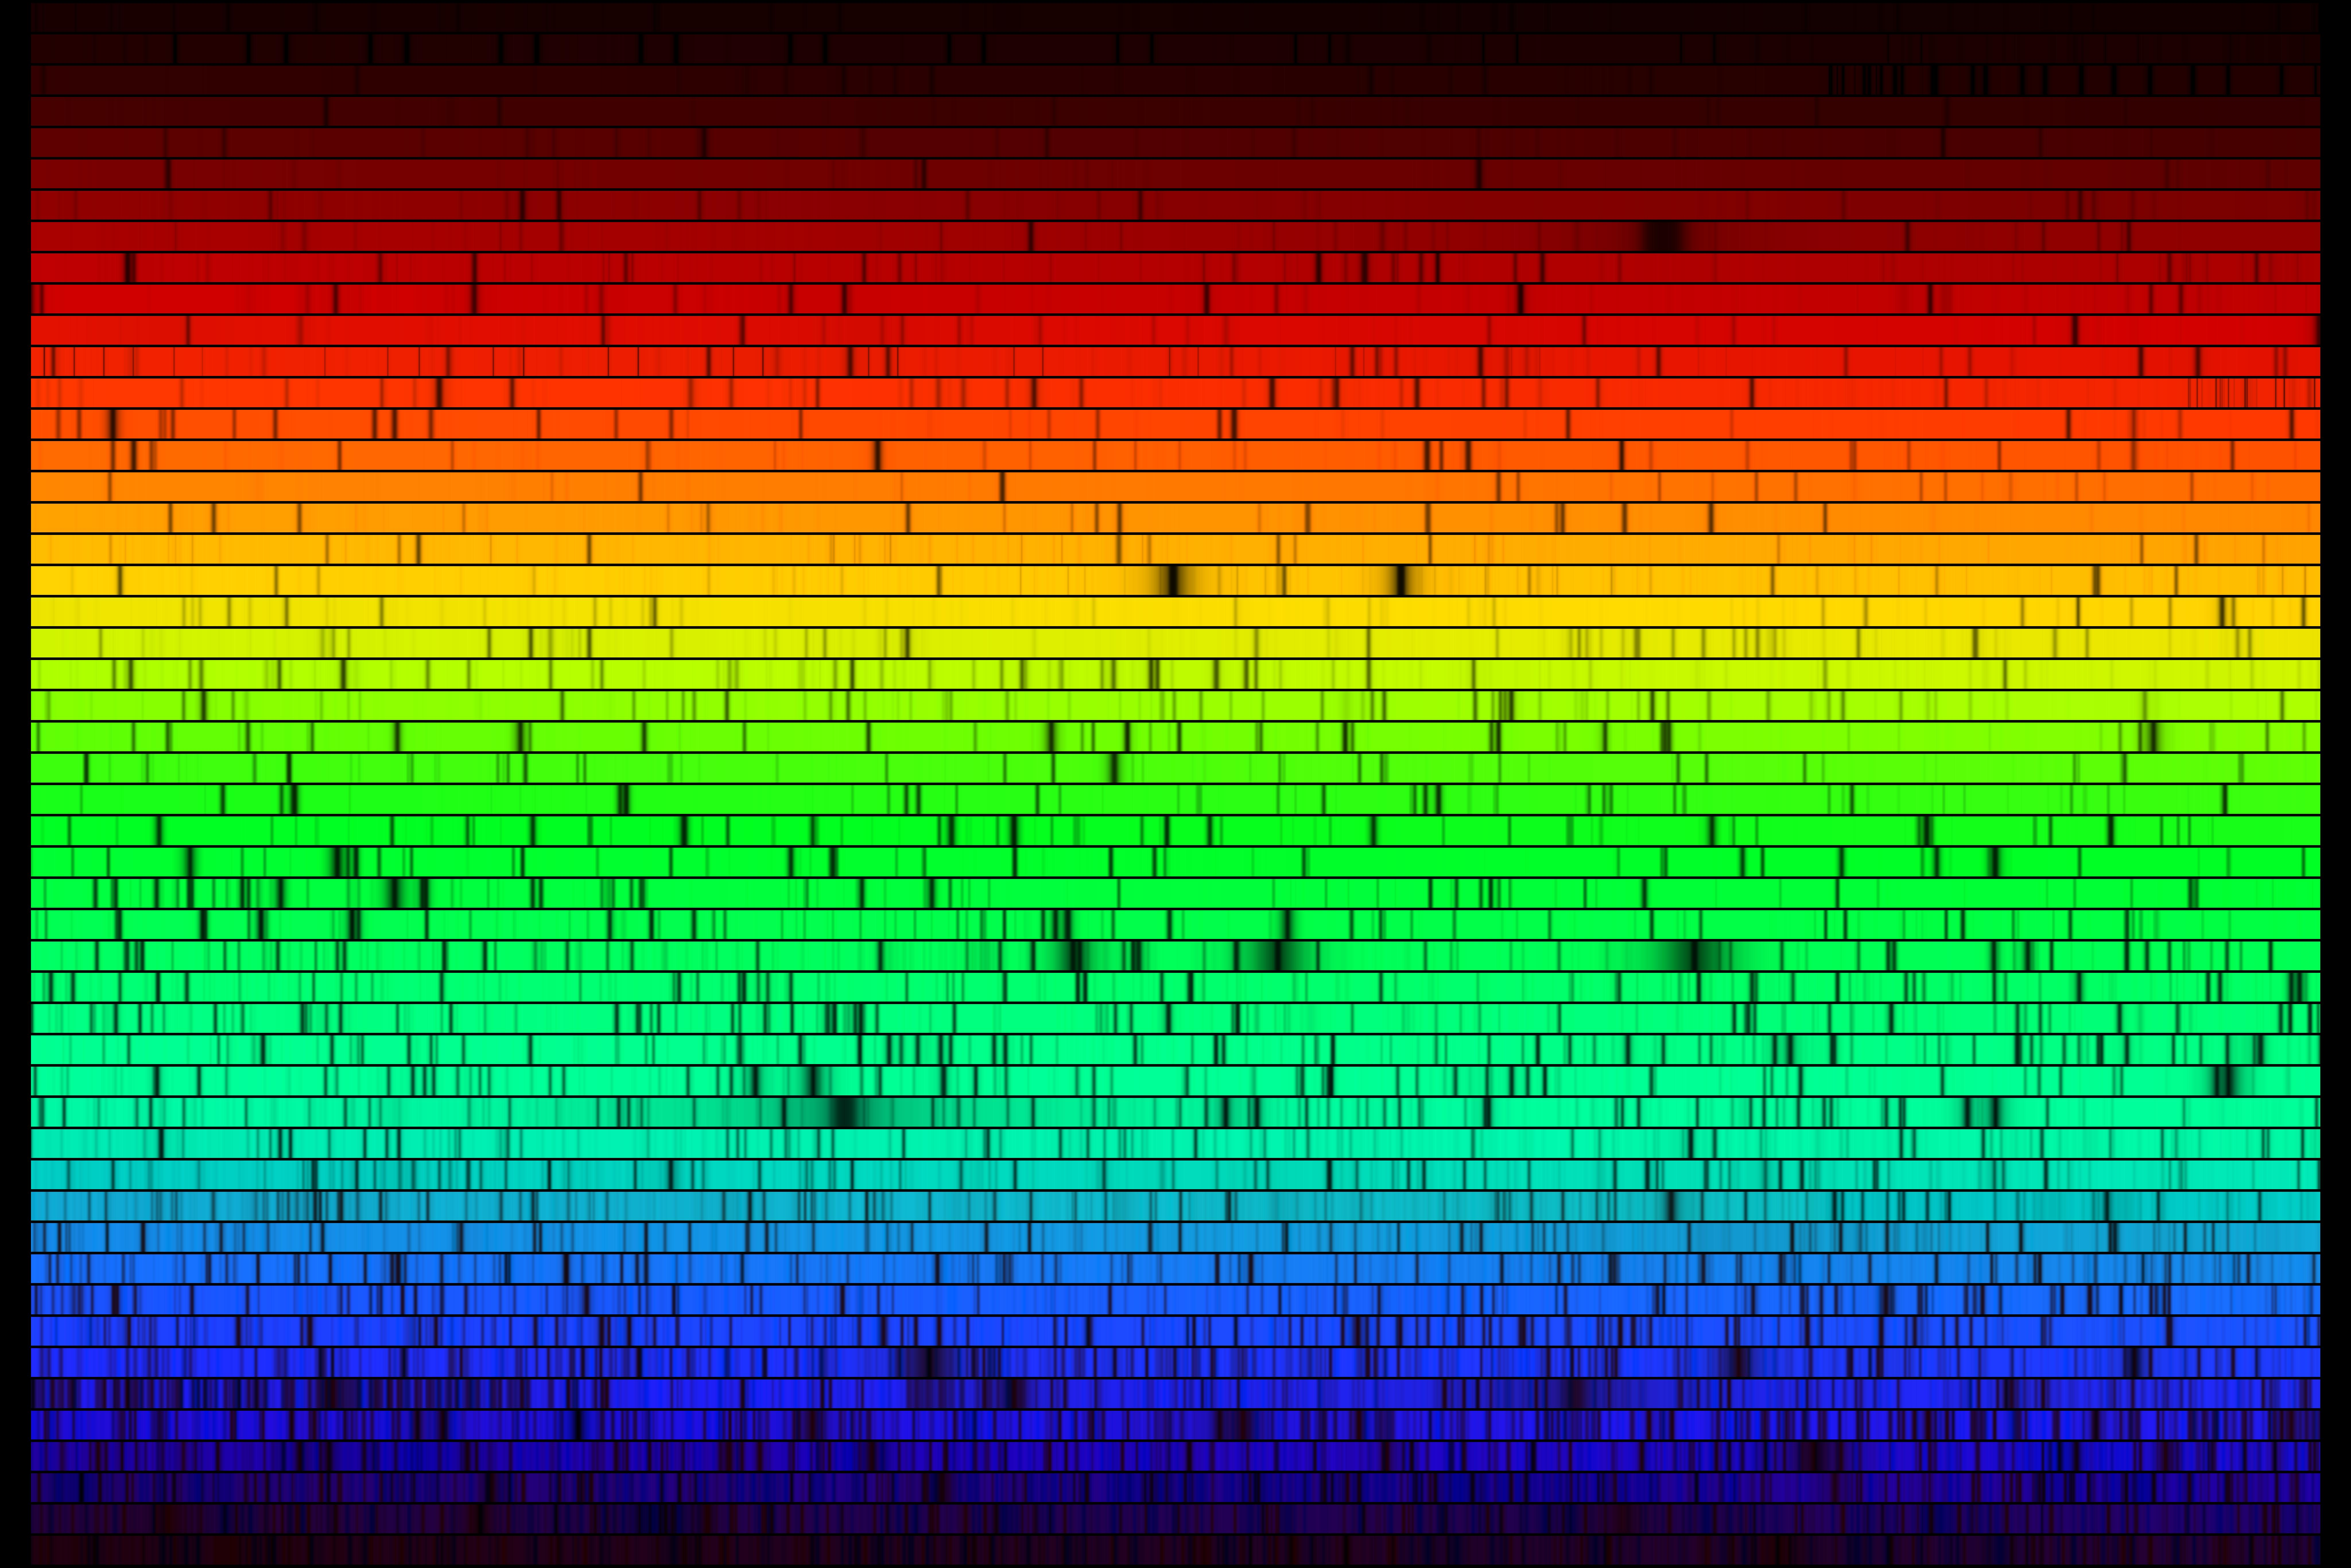
\includegraphics[width=\textwidth]{img/solarspectrum.jpg}
	\caption{The Solar Spectrum (Image by \href{https://solarsystem.nasa.gov/resources/390/the-solar-spectrum/}{NASA})}
	\label{solar_spectrum}
\end{figure}

\section{Large Spectroscopic Surveys}

Give list of large spectral archives focused on observation of QSOs.
Main archives are Ondřejov, LAMOST, Gaia (doesn't have spectra available yet)
and SDSS (similar to LAMOST, optical and IR, APOGEE survey).
Marginal archives are GALEX (ultraviolet), CALIFA or ESO MUSE.
Maybe GALAH.

Choose LAMOST and SDSS and tell why we have choosen them.

LAMOST is a stellar and extra-galactic spectroscopic survey.

SDSS is a spectroscopic and optical survey.

CALIFA is a spectroscopic survey of galaxies

\subsection{Sloan Digital Sky Survey}

Describe SDSS, its spectra and catalog of QSOs.

\begin{figure}
	% source https://solarsystem.nasa.gov/resources/390/the-solar-spectrum/
	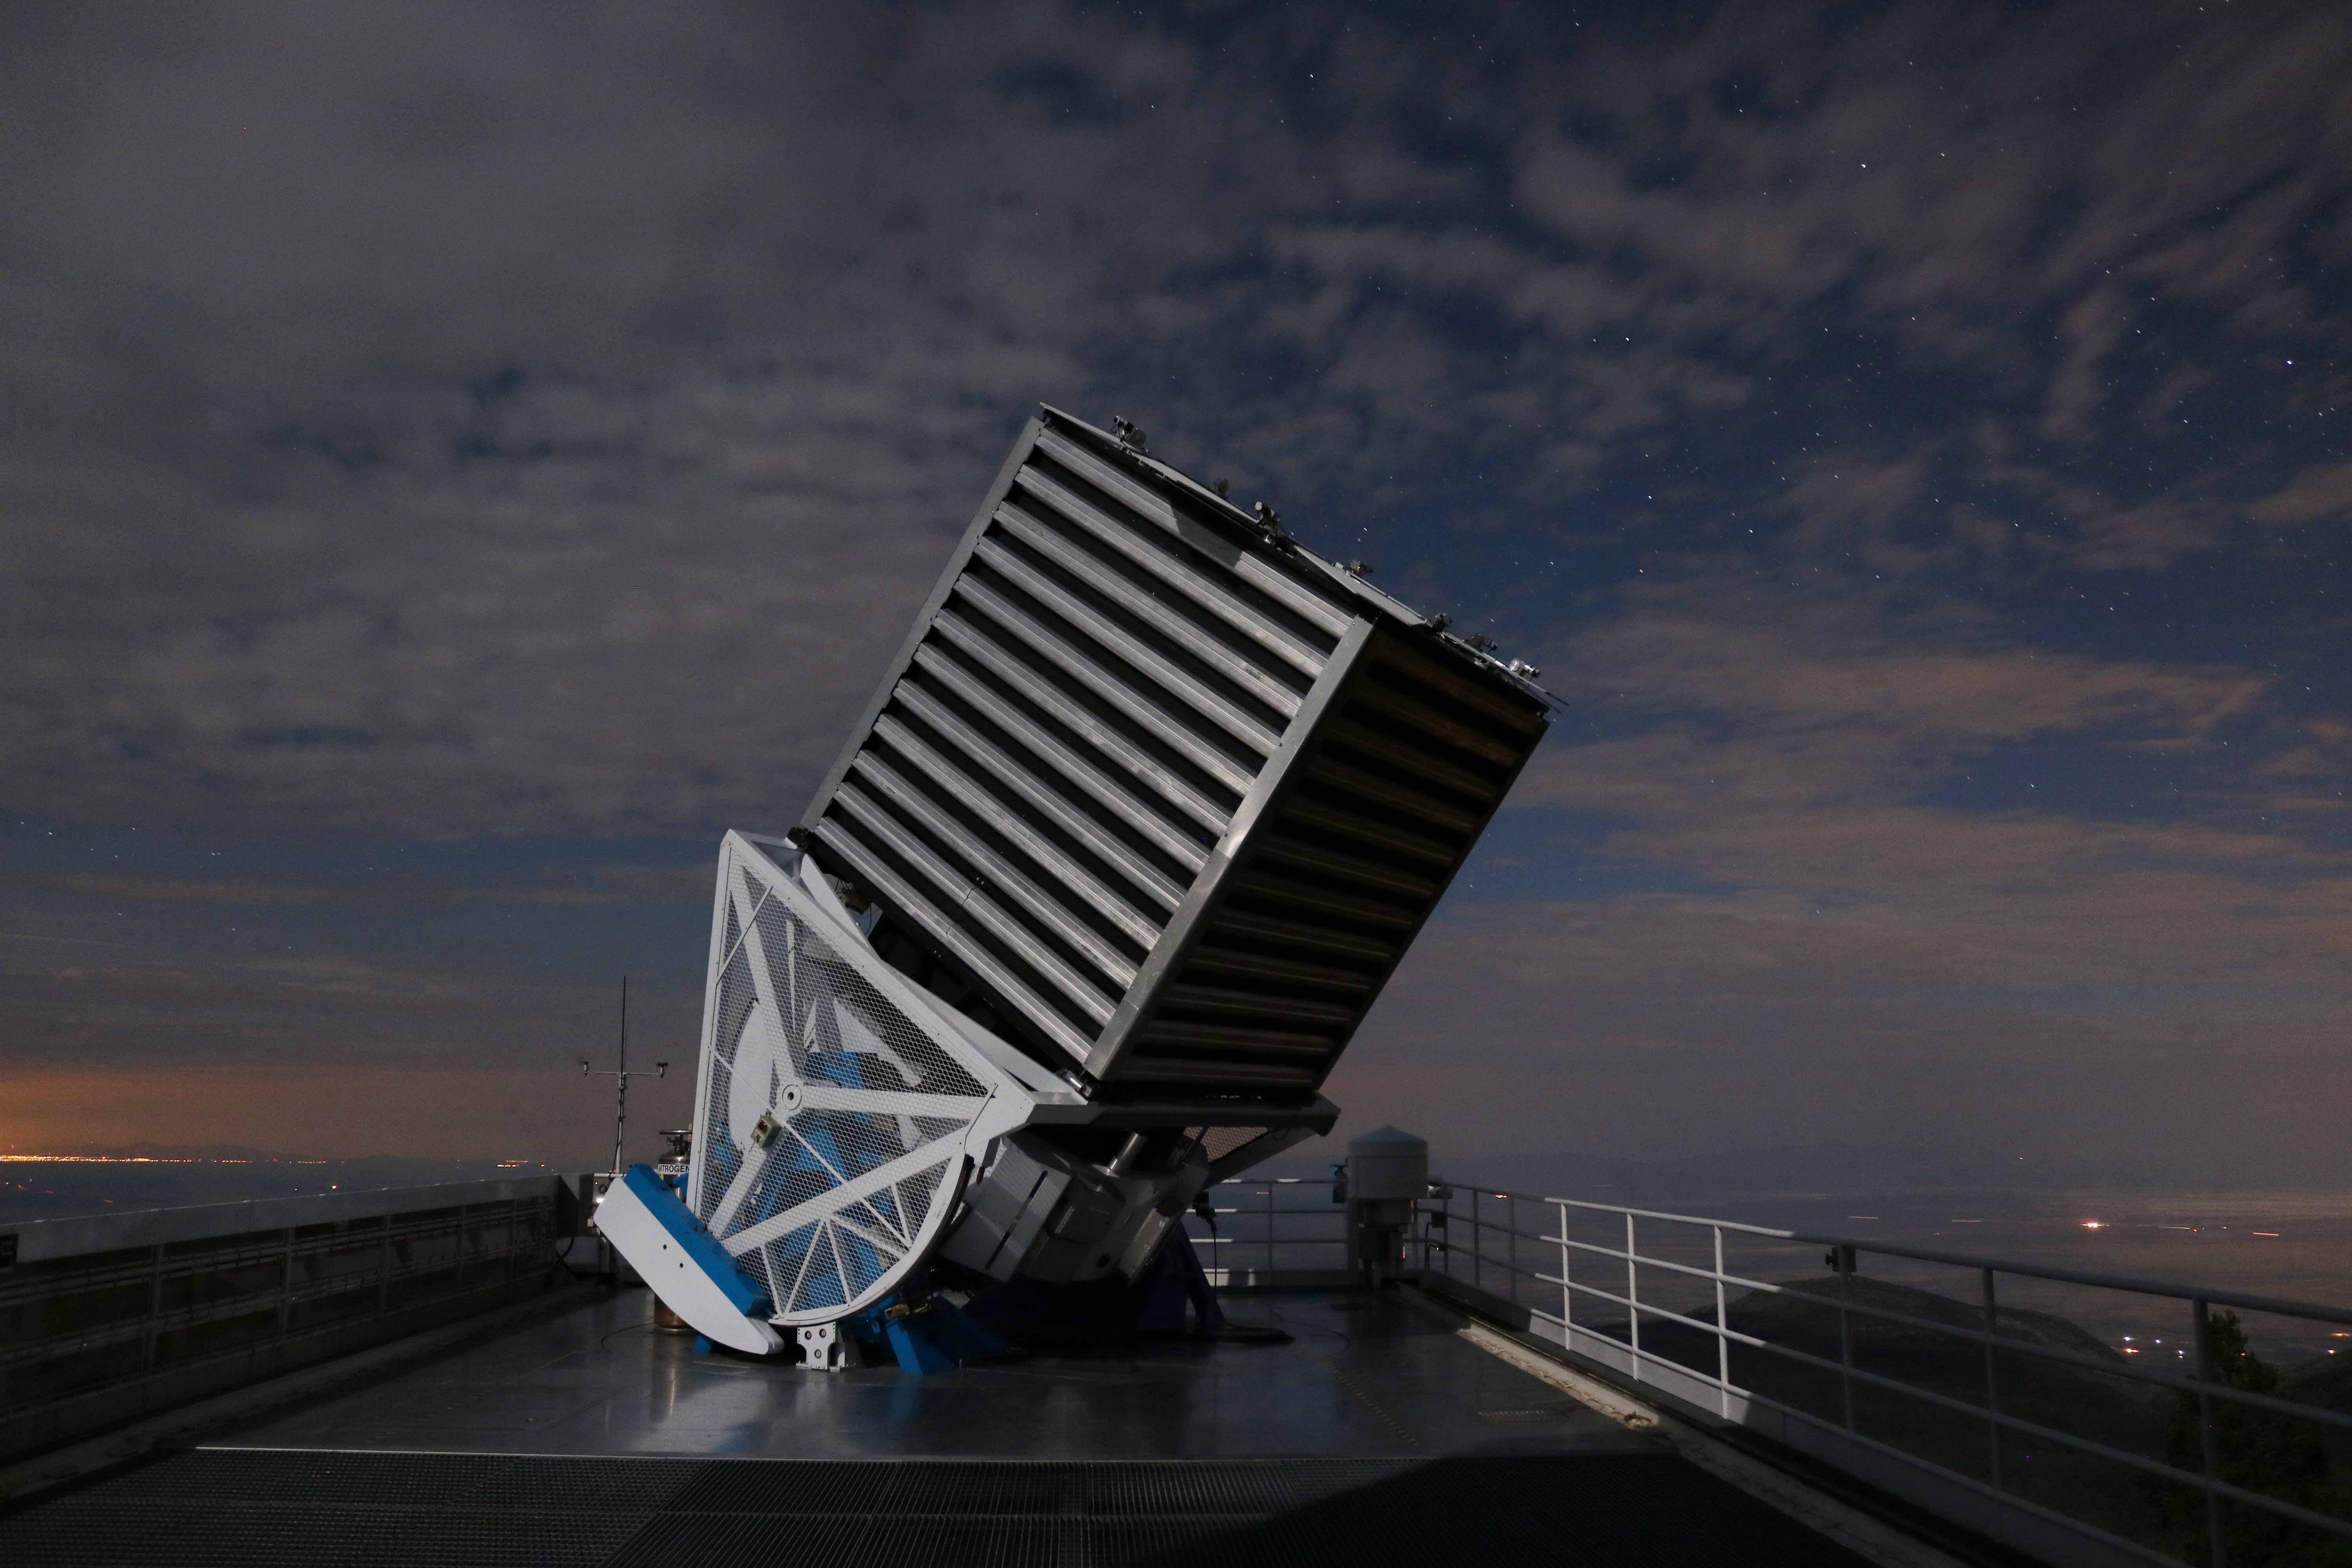
\includegraphics[width=\textwidth]{img/sdss_gaulme.jpg}
	\caption{The SDSS telescope at night (Image by Patrick Gaulme is licensed under CC BY 4.0)}
	\label{solar_spectrum}
\end{figure}

The SDSS DR14 Quasar Catalog described in~\cite{paris2018}.

\subsection{Large Sky Area Multi-Object Fiber Spectroscopic Telescope}

Describe LAMOST, its spectra and catalog of QSOs.

\section{Quasi-Stellar Objects}

Quasi-stellar (star-like) objects (also known as \textit{quasars} and abbreviated \textit{QSO}) are the most luminious \textit{active galactic nuleuses} (AGNs).~\cite{beckmann2013} % TODO add QSO and AGN to acronyms

The physical model is a supermassive black hole surrounded by a gaseous accretion disk.
A QSO generates energy by stress and friction in the disk outside ot the black hole because no light can escape the \textit{event horizont}.
The energy is in form of electromagnetic radiation and is the strongest in the ultraviolet band.
Moreover, QSOs exhibit big cosmological redshift.

QSOs were common in the early universe probably because galaxies have run out of matter: they stop to be so lumionious.
Therefore, QSOs help us to study the early universe.

There are different types of QSOs: radio-loud, radio-quiet, broad absorption-line, type II, red, optically violent variable, weak emission-line.

\begin{itemize}
	\item Physical definition of QSOs.
	\item Definition of QSOs according SDSS DR14Q.
	\item Why QSOs are interesting? Something as the expanding Universe.
	\item Why QSOs are suitable for experimenting with DA?
		QSOs have big redshift and CNNs are shift invariant.
		Searching for QSOs in different archives.
\end{itemize}

\begin{figure}
	% TODO give credit https://www.spacetelescope.org/images/potw1346a/
	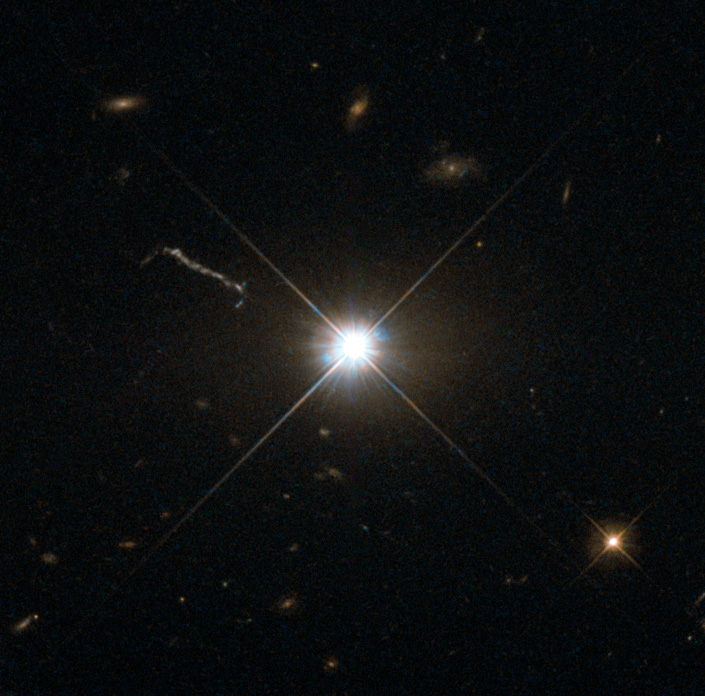
\includegraphics[width=\textwidth]{img/potw1346a.jpg}
	%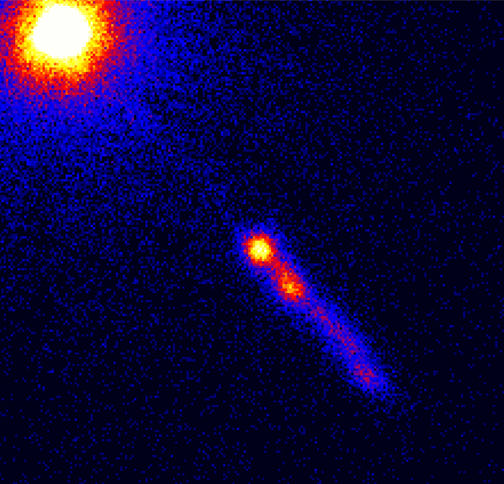
\includegraphics[width=0.5\textwidth]{img/0131_xray.jpg}
	\caption{
		Best image of bright quasar 3C 273
		(Image by \href{https://www.spacetelescope.org/images/potw1346a/}{ESA/Hubble} is licensed under CC BY 4.0)
		}
	\label{3c_273}
\end{figure}

% TODO include https://chandra.harvard.edu/photo/2000/0131/index.html
% TODO include 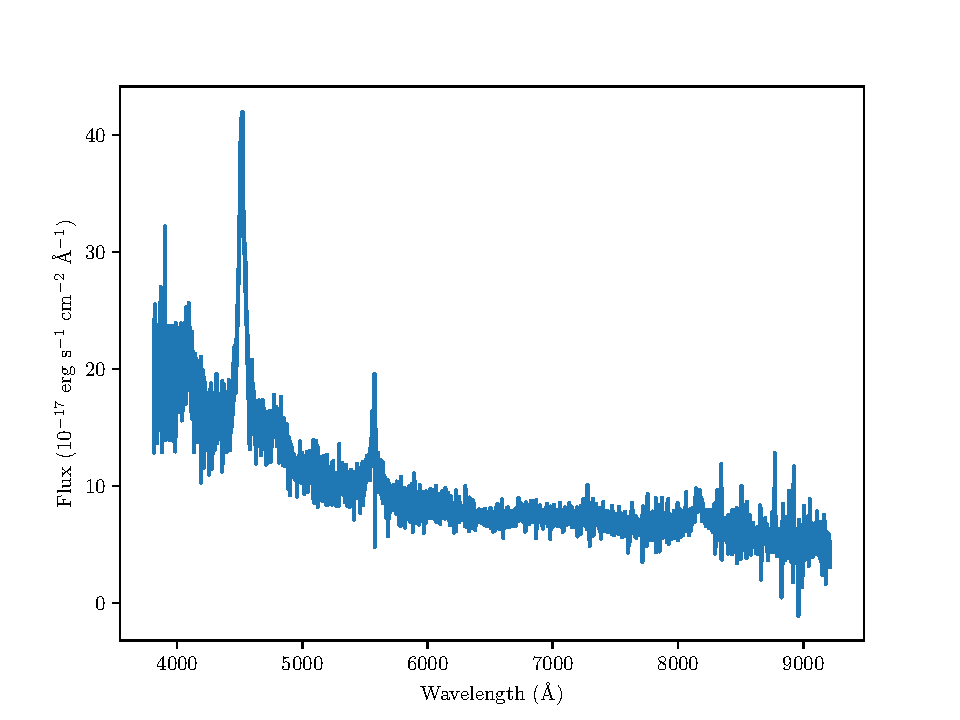
\includegraphics[width=\textwidth]{img/spec_3c_273.pdf}

\section{Comparison of the Spectral Data}

Compare instruments, data and sky coverage.

Investigate the structure of data space in selected datasets (dimensionality reduction).

\chapter{Experiments: Application of Neural DA to Spectral Data}
\label{exp_chapter}

\section{Results without use of Neural DA}

\section{Benefits of Neural DA: Analysis and Visualisation of Results}

Apply domain adaptation to the selected data
and prepare visualisation of results.

\chapter{Conclusion}

\section{Discussion of Performance}

Discuss the precision performance and scalability of various solutions.

\section{Future Plans}

Suggest future improvements.

\bibliographystyle{iso690}
\bibliography{references}

\appendix

\chapter{Acronyms}
\begin{description}
    \item[LAMOST] Large Sky Area Multi-Object Fiber Spectroscopis Telescope
\end{description}

\chapter{Contents of Enclosed CD}

\begin{figure}
\dirtree{%
    .1 README.md\DTcomment{the file with CD contents description}.
    .1 src\DTcomment{the directory of source codes}.
    .2 latex\DTcomment{the directory of \LaTeX{} source codes of the thesis}.
    .1 thesis.pdf\DTcomment{the thesis text in PDF format}.
}
\end{figure}

\end{document}
